

I/O requests handled by the ESD middleware are received via the ESDM interfaces as they are described in \Cref{sec: viewpoints/logical/semantics}.
In most cases, these requests must collect additional information / identify multiple fragments to fulfil a request.
The ESDM scheduler is responsible to progress potentially operations, coordinate requests, and invoke the appropriate handlers.
In particular, the scheduler will consult the layout component to determine which fragments to create or use and which storage backends to use.
For a discussion of the decision process for a mapping of a I/O request to backends refer to \Cref{component: layout} on the layout component.


%%%%%%%%%%%%%%%%%%%%%%%%%%%%%%%%%%%%%%%%%%%%%%
\subsection{Logical View}

\begin{figure}
	\centering
	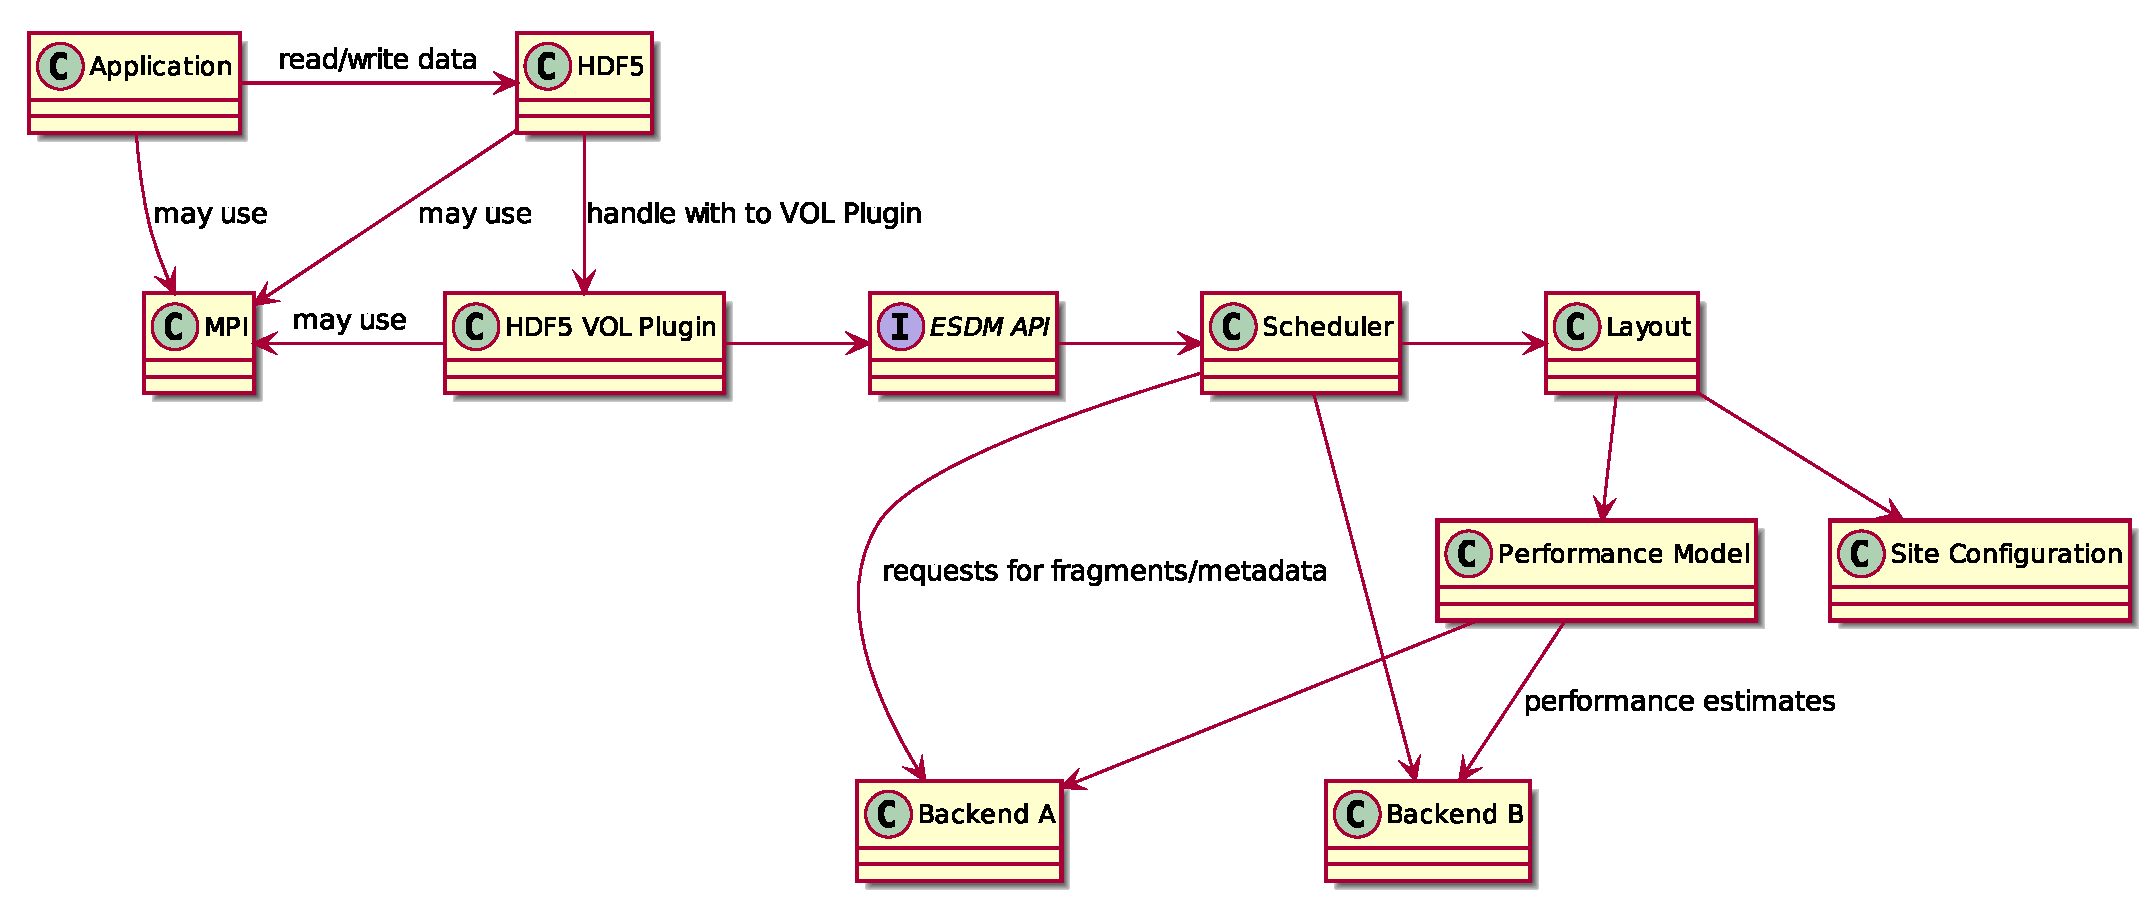
\includegraphics[width=\linewidth]{esdm-components/scheduler/logical.eps}
	\caption{Logical view to the ESDM scheduling component.
	Applications issue requests that are then handled and delegated by the Scheduler to other components.}
	\label{fig:esdm scheduler logical view}
\end{figure}

The scheduling component has two core responsibilities:

\begin{enumerate}
	\item Accept incoming operations from the ESDM Interface and delegate them to handlers possibly in separate threads.
	\item Coordinate the progressing of complex operations and the response/completion of the operations.
\end{enumerate}

In \Cref{fig:esdm scheduler logical view}, the relation of the scheduling component (scheduler) to the rest of the ESDM architecture is illustrated.
An application will issue a request which is queued to the scheduler for consideration.
The scheduler will delegate the request to the layout component which will also consult a performance model to make a decision (refer to \Cref{component: layout} for details).
The resulting operations to internal objects (fragments) may then require a number of requests to various ESDM backends.
These subsequent operations are also coordinated by the Scheduler.




%%%%%%%%%%%%%%%%%%%%%%%%%%%%%%%%%%%%%%%%%%%%%%
\subsection{Process View}

\begin{figure}
	\centering
	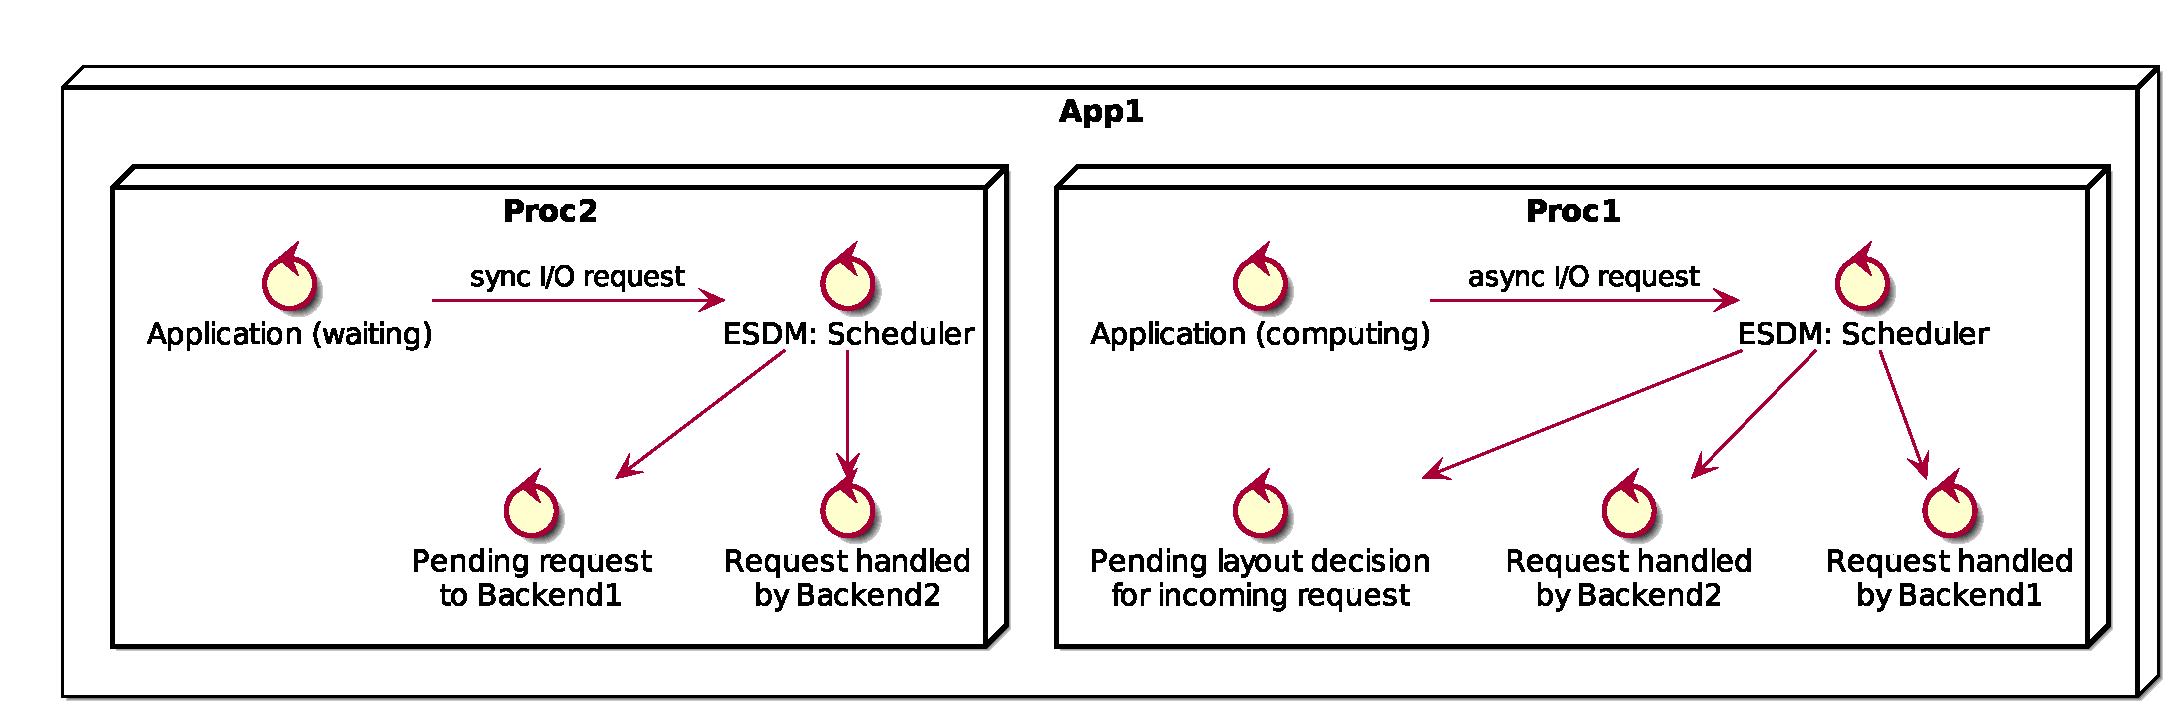
\includegraphics[width=\linewidth]{esdm-components/scheduler/process.eps}
	\caption{Process view to the ESDM scheduling component. Applications should when possible issue I/O asynchronously. In either situation the ESDM scheduler may execute multiple threads in parallel to gather or flush fragments to the backends or make a layout decision.}
	\label{fig:esdm scheduler process view}
\end{figure}

The scheduling component is responsible for the bulk of concurrency within the ESDM.
Requests arrive and have to be dispatched to appropriate handlers such as the layout component or a ESDM backend.
This approach is necessary so the ESDM remains responsive as new requests arrive and because it considerably can speed up the reconstruction/flushing of requested views.
\Cref{fig:esdm scheduler process view} provides a overview to active and waiting process as requests are being handled by the ESDM. Notice that Process 1 handles a asynchronous request which allows the application to continue computation, while Process 2 depicts the synchronous case.
In both cases the ESDM will try to perform the domain reconstruction concurrently.


%%%%%%%%%%%%%%%%%%%%%%%%%%%%%%%%%%%%%%%%%%%%%%
\subsection{Physical View}

\begin{figure}
	\centering
	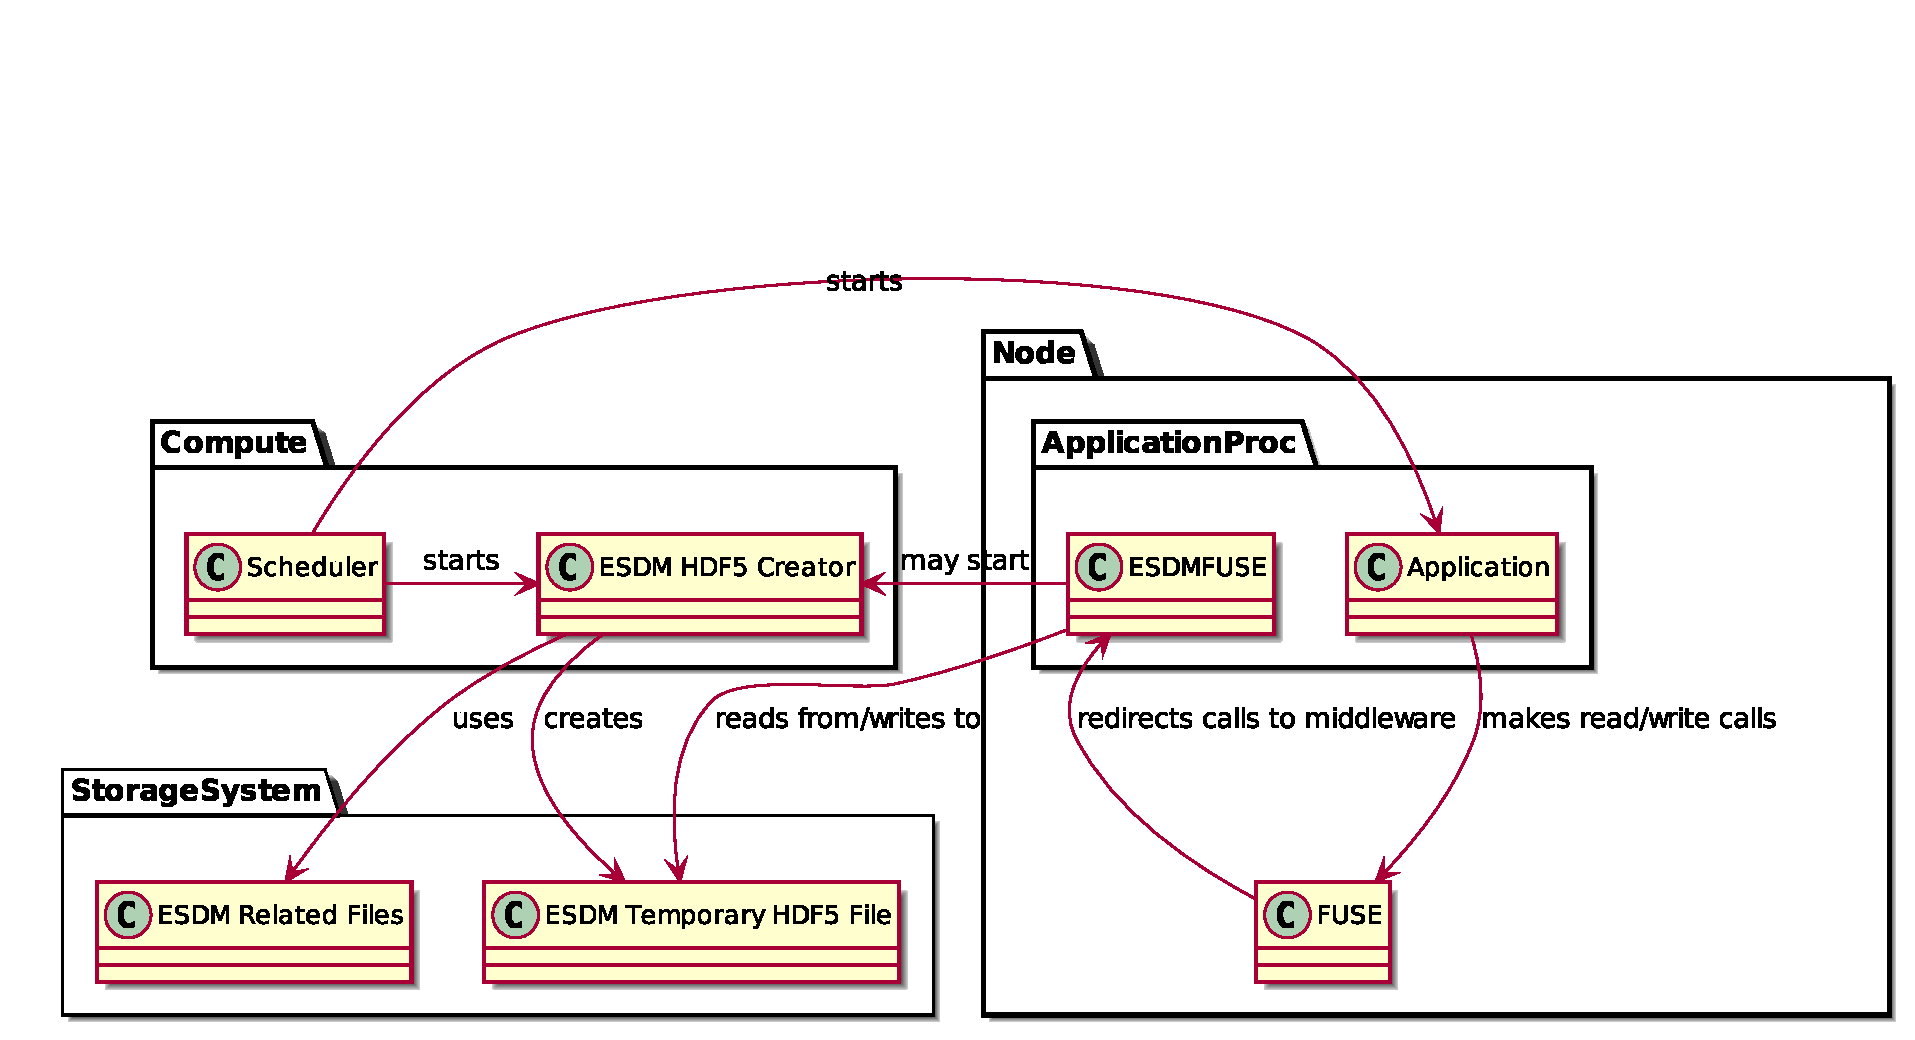
\includegraphics[width=\linewidth]{esdm-components/scheduler/physical.eps}
	\caption{Physical view to the ESDM scheduling component. The scheduler is only active within the application process.}
	\label{fig:esdm scheduler physical view}
\end{figure}


An application may be spread out across many nodes and on each node have multiple running processes.
Each running process that is using ESDM as a scheduling component running as is illustrated in \Cref{fig:esdm scheduler physical view}.
Within ESDM, only the scheduler starts threads.
The ESDM scheduler does not directly expect any modifications or prerequisites from the storage system, but changes to the configuration of the storage system should be reflected in the site configuration.

%
%%%%%%%%%%%%%%%%%%%%%%%%%%%%%%%%%%%%%%%%%%%%%%%
%\subsection{Development View}
%
%\begin{figure}
%	\centering
%	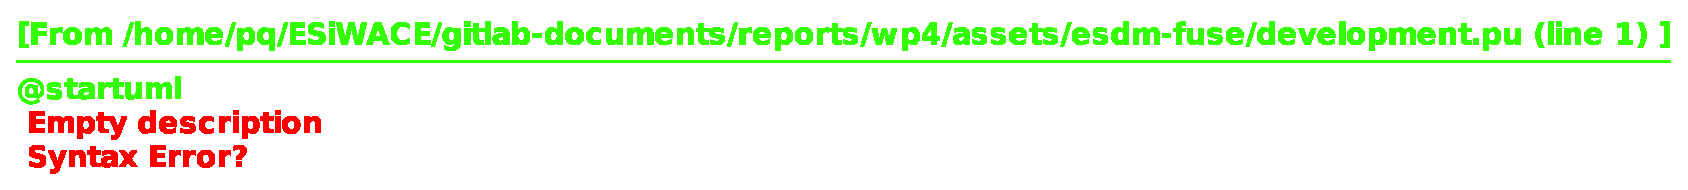
\includegraphics[width=\linewidth]{esdm-component/scheduler/development.eps}
%	\caption{}
%	\label{fig:esdm scheduler development view}
%\end{figure}
%
%\Cref{fig:esdm scheduler development view}
%
%
